\documentclass{beamer}
\usetheme{Warsaw}

\usepackage{epsfig}
% \usepackage{beamerthemesplit} // Activate for custom appearance

\title{Mapping neuronal networks}
\subtitle{Progress Talk}
\author{Cathal Cooney}
\institute{School of Maths, Trinity College Dublin}
\date{\today}

\begin{document}
\frame{\titlepage}

\section[Outline]{}
\frame{\tableofcontents}


\section{Motivation}
\frame
{
\frametitle{The Brain is a Network}
\begin{itemize}
\item The brain is a network of neurons.
\item Want to be able to determine the network structure.
\pause
\item Possible to dye neurons to view physical structure.
\end{itemize}
}

\frame
{
\frametitle{Flow of information}
\begin{itemize}
\item What about the functional structure?
\pause
\item We want to pick out how information passes through the brain.
\pause
\item Is there a "small-world" structure?
\pause
\item What data do we need to determine the structure?
\end{itemize}
}

\frame
{
\frametitle{Population Coding}
Some theories say that chains of neurons that fire each other appear in the network.
\pause
\begin{itemize}
\item However, single neurons are very noisy.
\pause
\item Shadlen \& Newsome [1998] showed that a population of neurons in a network can bear a resemblance to a background rate.
\item A population of irregular neurons fire with a regular rate overall.
\pause
\item So, perhaps we should look for neurons that work together?
\end{itemize}
}

\section{Incremental Mutual Information}

\frame
{
\frametitle{Entropy}
What is entropy?
\bigskip
\pause

It is the measure of uncertainty of a random variable or data series X.
$$
H(X) = \sum_{x \in X}  -p(x)\ln (p(x))
$$
}

\frame
{
\frametitle{Mutual Information}
We get a measure for similarity between two data series.

$$I(X,Y) = H(X) - H(X|Y) = H(Y) - H(Y|X)$$
\pause
\begin{itemize}
\item We can use this for comparing spike-trains by binning them into binary vectors.
\pause
\item If we offset these binary vectors, we can investigate if there is a causal link between two spike-trains.
\end{itemize}
}

\frame
{
\frametitle{Incremental Mutual Information}
However, spike-trains are very noisy, so Mutual Information doesn't tell the whole story.
\pause

We can give more context to the probability distribution, by looking forward and backward a few steps in both X and Y.
\pause

\bigskip
In 2010 Singh and Lesica defined the Incremental Mutual Information (IMI):
$$
\begin{array}{lll} \Delta I_{XY}(\delta) & = & H(X[n] | X_p[n], X_f[n], Y_p[n-\delta],Y_f[n-\delta]) \\
& - & H(X[n] | Y[n-\delta], X_p[n], X_f[n], Y_p[n-\delta],Y_f[n-\delta]) \end{array}
$$ 
}

\section{Directed networks}
\frame
{
Directed networks have adjacency matrices:
$$
A_{ij} = \left\{ \begin{array}{ll} 1 & \text{ if there is a link of from node $j$ to node $i$.}\\
0 & \text{ otherwise.}\end{array} \right.
$$
\pause
\begin{itemize}
\item<1-> Directed networks don't cluster as well as undirected networks. 
\item<2-> What information do we want from the directed network?
\end{itemize}
}
\subsection{Bibliographic Coupling}
\frame
{
\frametitle{Bibliographic Coupling}
One way of symmetrising the network is to view the bibliographic couplings of the network.
$$
B_{ij} = \sum_{k} A_{ki}A_{kj}
$$
\pause
This tells us how many common nodes that nodes $i$ and $j$ point at.
\pause
We can alter it for weighted networks by considering the amount of common output from nodes $i$ and $j$.
\pause
$$
B_{ij} = \sum_k \min (A_{ki}A_{kj})
$$

}

\subsection{Cocitation Couping}
\frame
{
\frametitle{Cocitation Coupling}
The cocitation coupling tells us the other side of the story.
$$
C_{ij} = \sum_k A_{ik}A_{jk}
$$
\pause
This is the number of common nodes that point at nodes $i$ and $j$.
\pause
Again, for weighted networks, can alter:
$$
C_{ij} = \sum_k \min (A_{ik}A_{jk})
$$
\pause
This is the common input to nodes $i$ and $j$.
}

\section{Results}
\frame
{
\frametitle{Algorithm}
By combining these ideas, of IMI and bibliographic coupling we get a process for mapping networks of neurons.
\begin{itemize}
\item<1-> We use the peak IMI pairwise on spike-trains to get a direction and weight of influence, forming a weighted directed network.
\item<2-> Get undirected networks by using the bibliographic and cocitation couplings.
\item<3-> Using Newman's modularity clustering algorithm, we get functional clusters of the network.
\item<4-> Refer back to directed network to determine the information flow through the network.
\end{itemize}
}

\frame
{
\frametitle{Model Network}
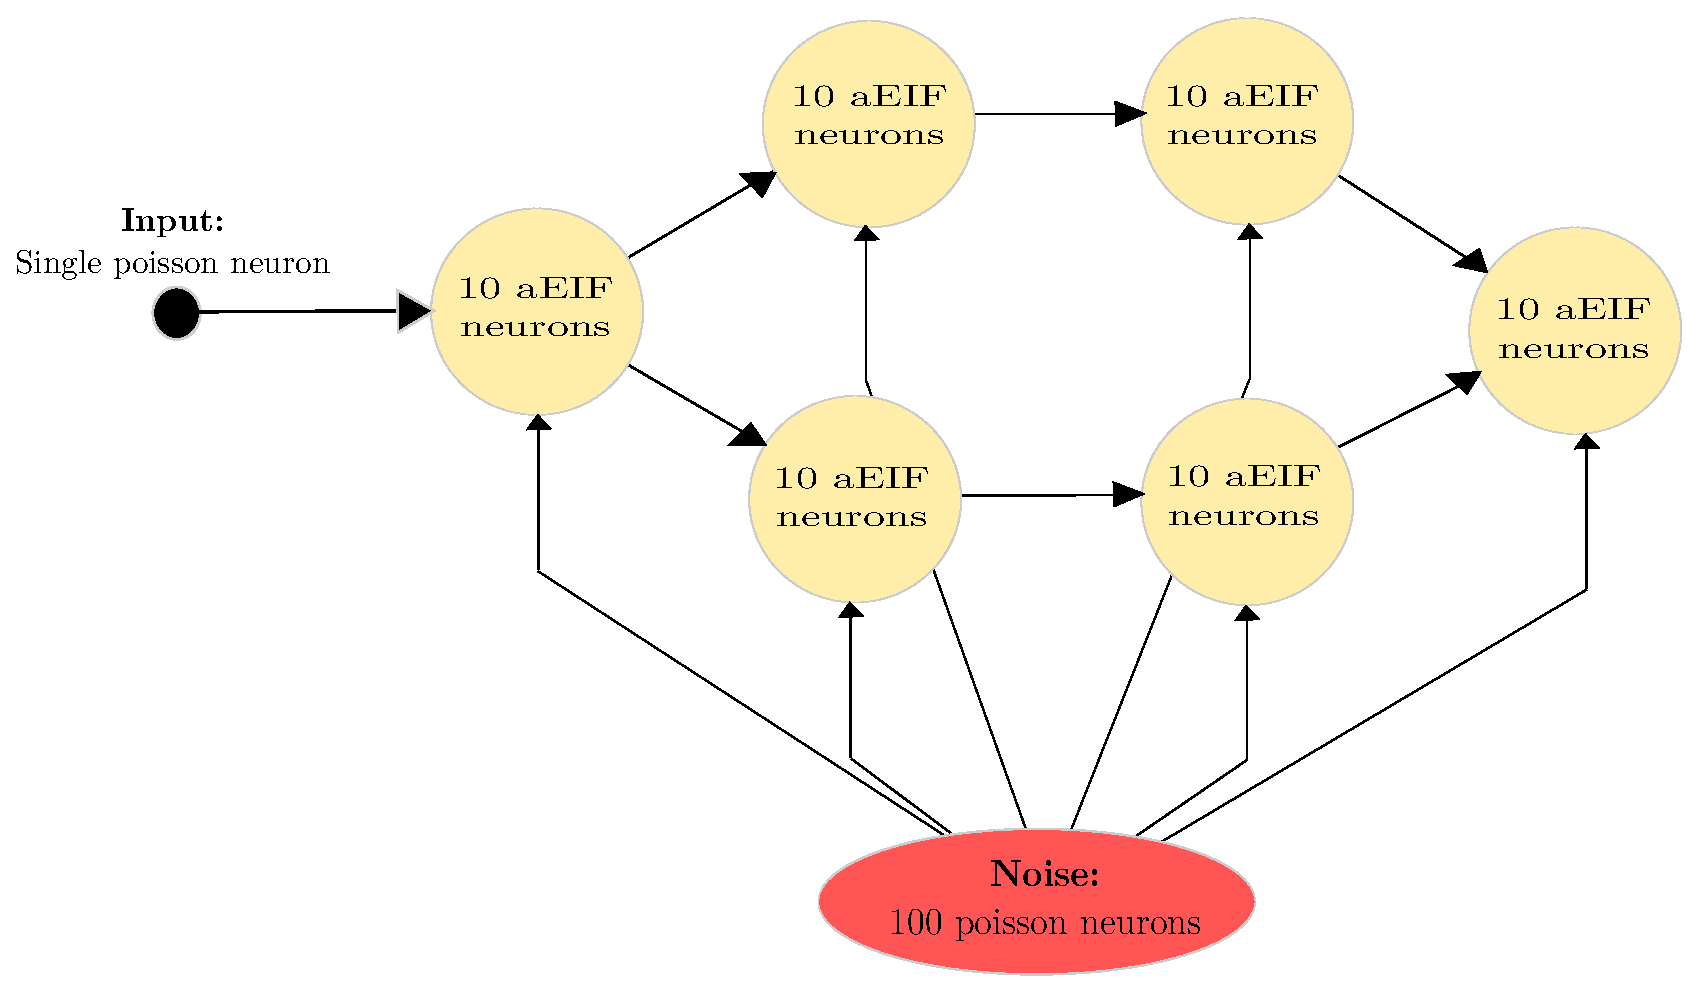
\epsfig{file=modelnetwork.eps, width=0.9\textwidth}
}

\frame
{
\frametitle{Connection Matrix}
\begin{center}
\epsfig{file=weightmatrix.eps, height=0.8\textheight}
\end{center}
}

\frame
{
\frametitle{IMI matrices as noise increases}
\begin{center}
\begin{tabular}{llll}
\epsfig{file=IMI1.eps,height=0.2\textheight} & \epsfig{file=IMI2.eps,height=0.2\textheight} & \epsfig{file=IMI3.eps,height=0.2\textheight} & 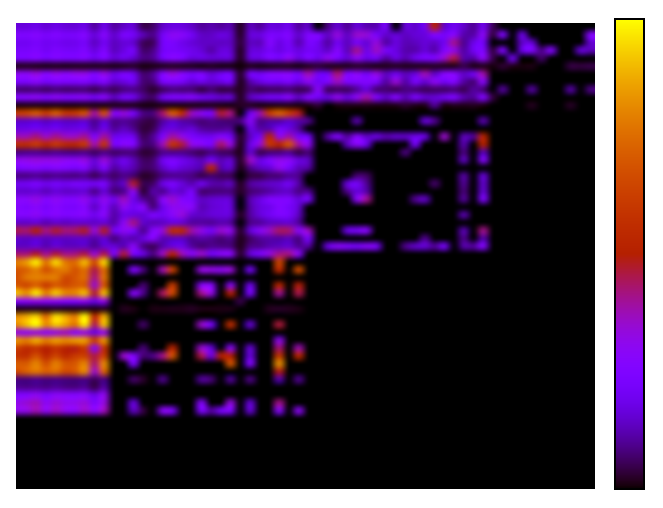
\epsfig{file=IMI4.eps,height=0.2\textheight} \\
\epsfig{file=IMI5.eps,height=0.2\textheight} & \epsfig{file=IMI6.eps,height=0.2\textheight} & \epsfig{file=IMI7.eps,height=0.2\textheight} & \epsfig{file=IMI8.eps,height=0.2\textheight} \\
\epsfig{file=IMI9.eps,height=0.2\textheight} & \epsfig{file=IMI10.eps,height=0.2\textheight} & \epsfig{file=IMI11.eps,height=0.2\textheight} & \epsfig{file=IMI12.eps,height=0.2\textheight}\\
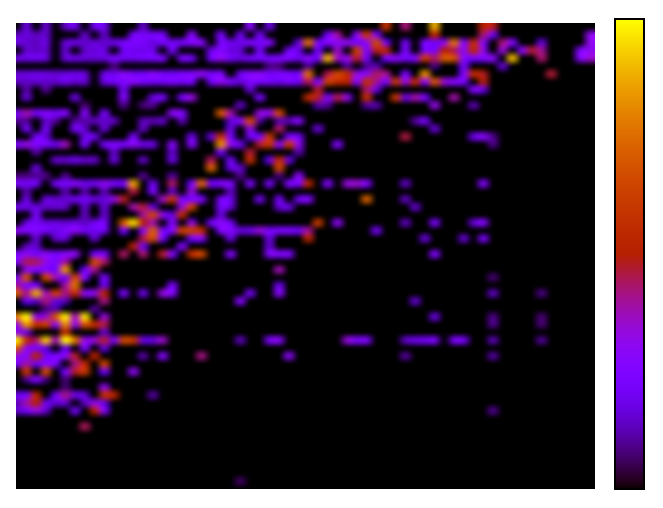
\epsfig{file=IMI13.eps,height=0.2\textheight} & \epsfig{file=IMI14.eps,height=0.2\textheight} & \epsfig{file=IMI15.eps,height=0.2\textheight} & \epsfig{file=IMI16.eps,height=0.2\textheight}
\end{tabular}
\end{center}
}

\frame
{
\frametitle{Directed Network}
\begin{center}
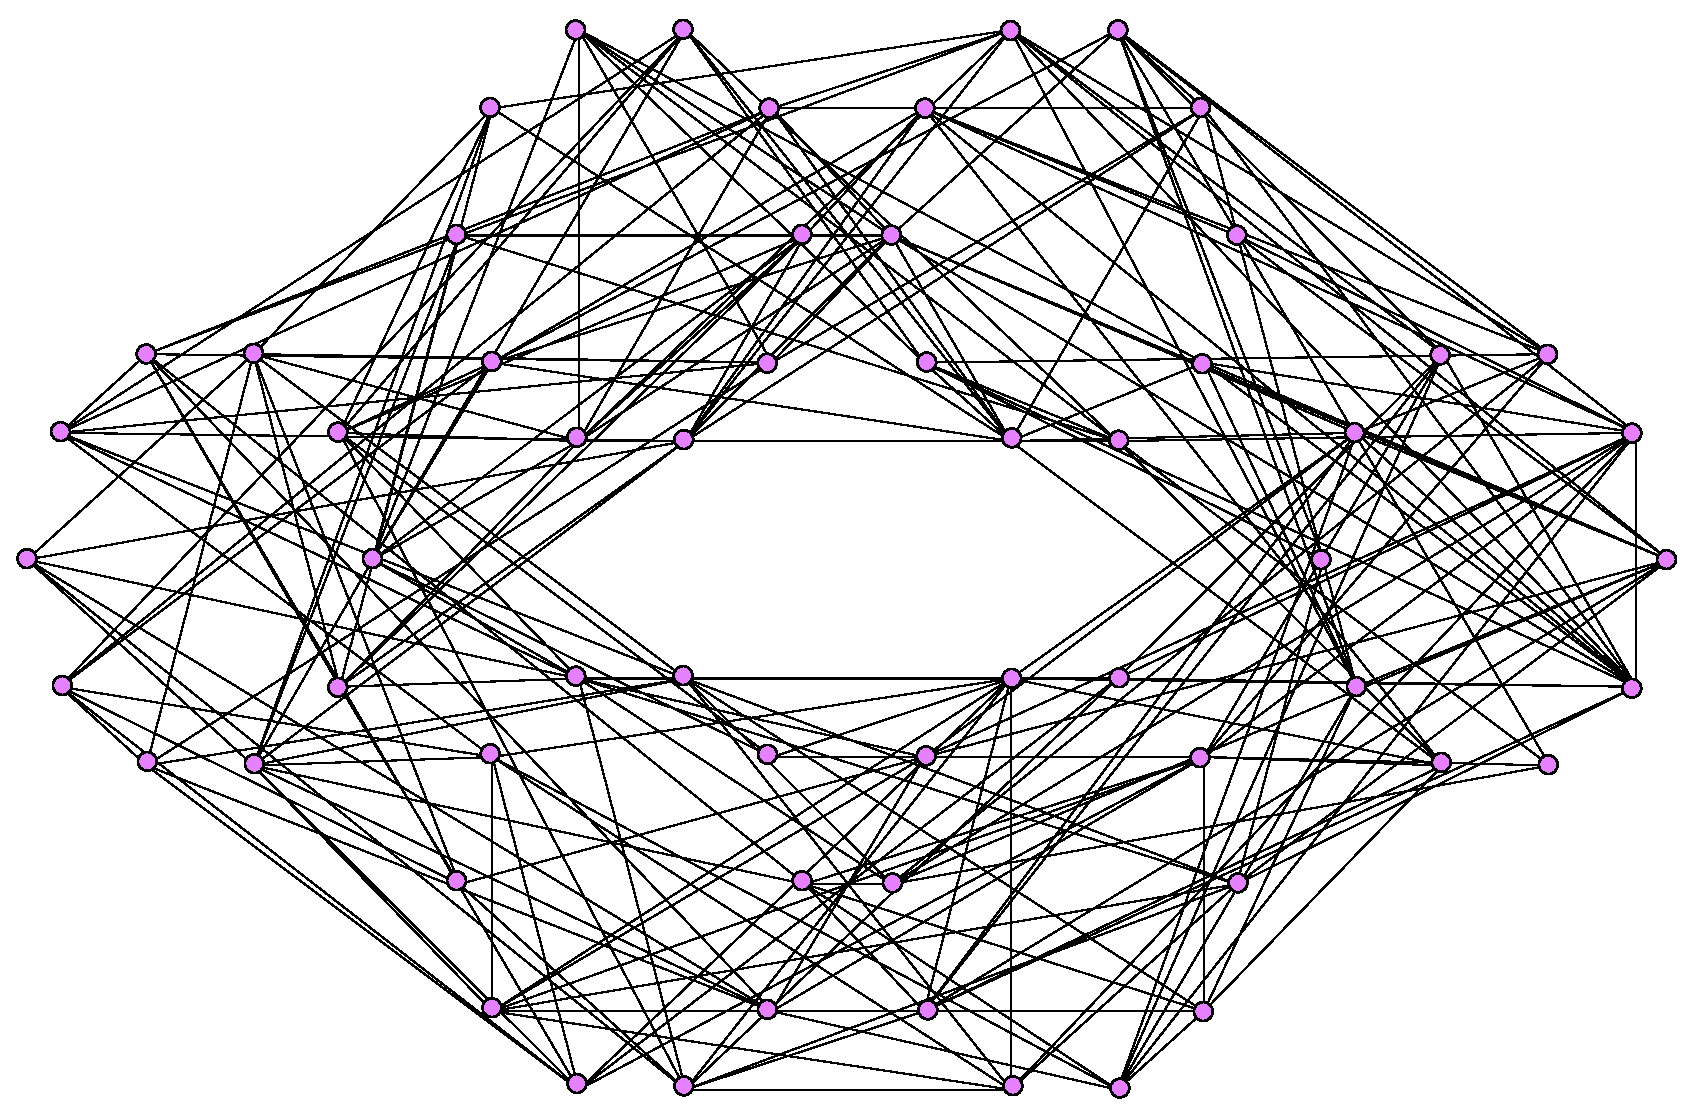
\epsfig{file=directednetnodes.eps, width=0.75\textwidth}
\end{center}
}
\frame
{
\frametitle{Biliographic Coupling Network}
\begin{center}
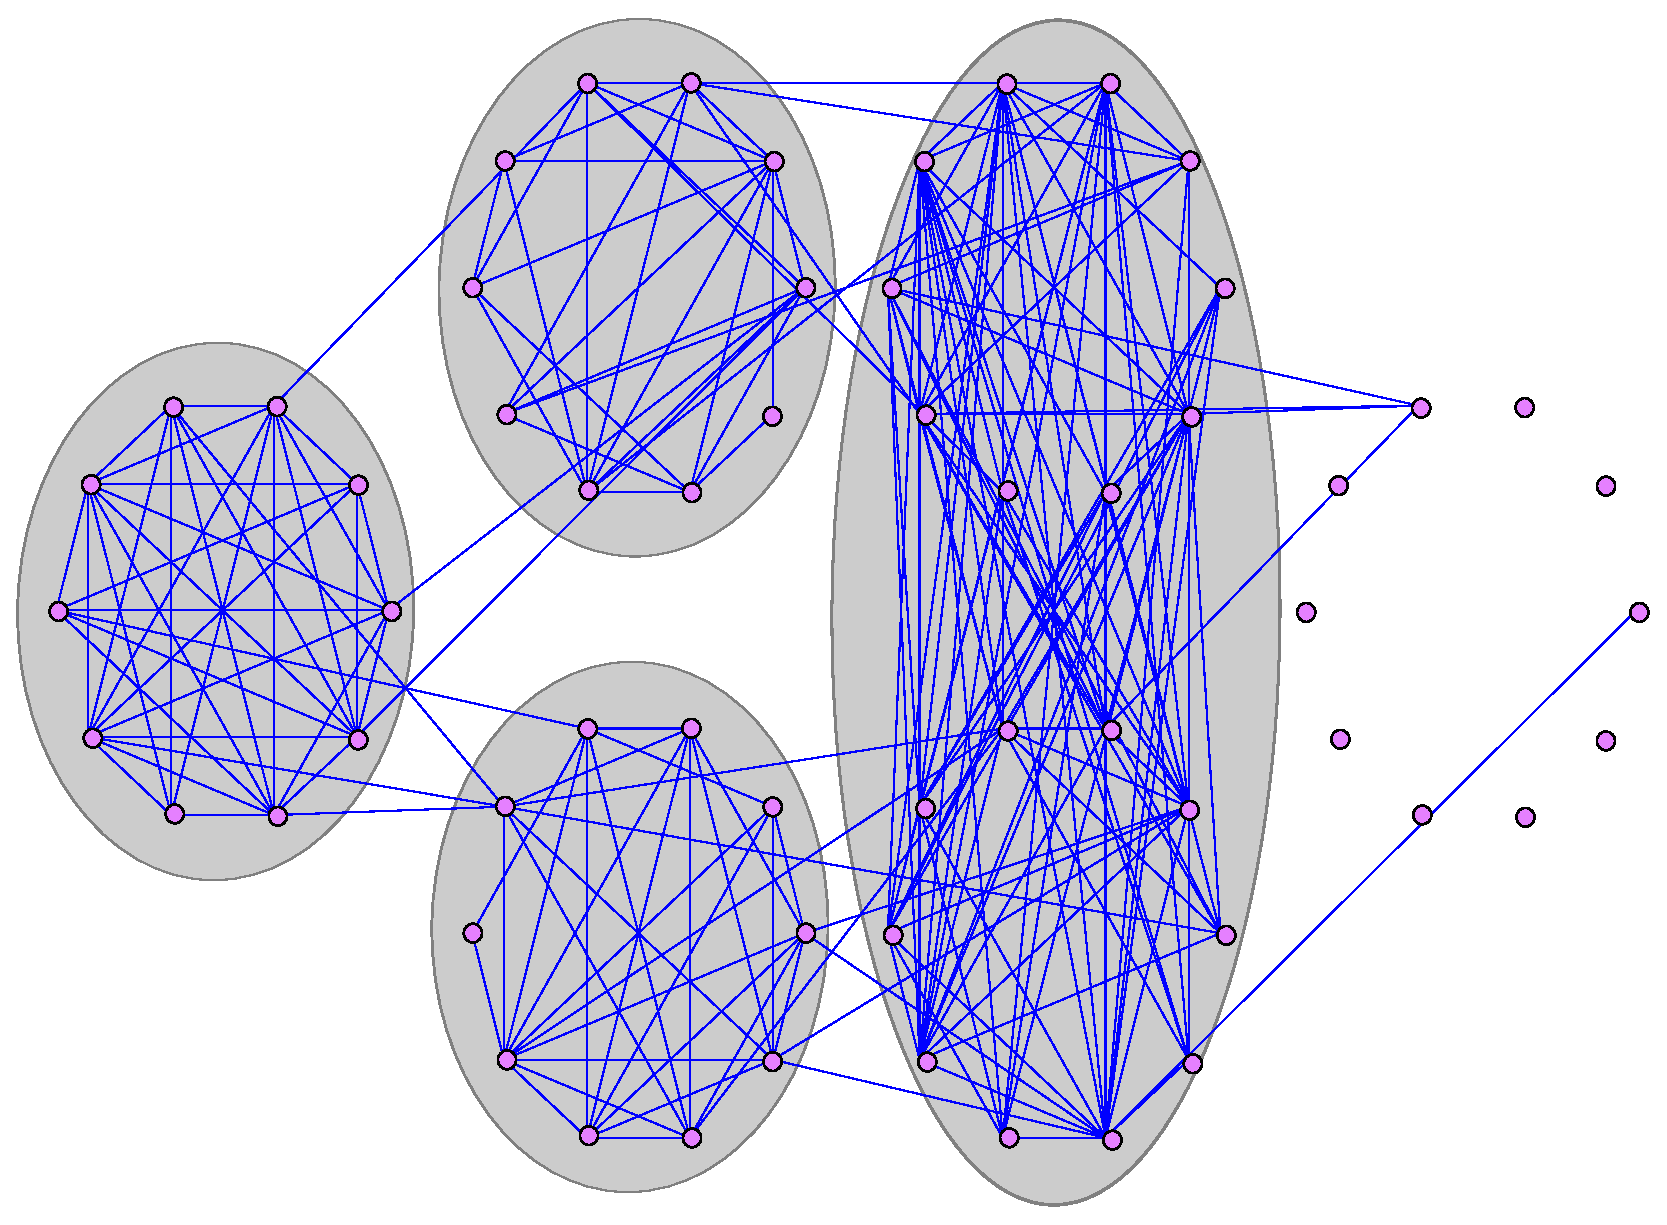
\epsfig{file=clustbibnetnodes.eps,width=0.75\textwidth}
\end{center}
}

\frame
{
\frametitle{Cocitation Coupling Network}
\begin{center}
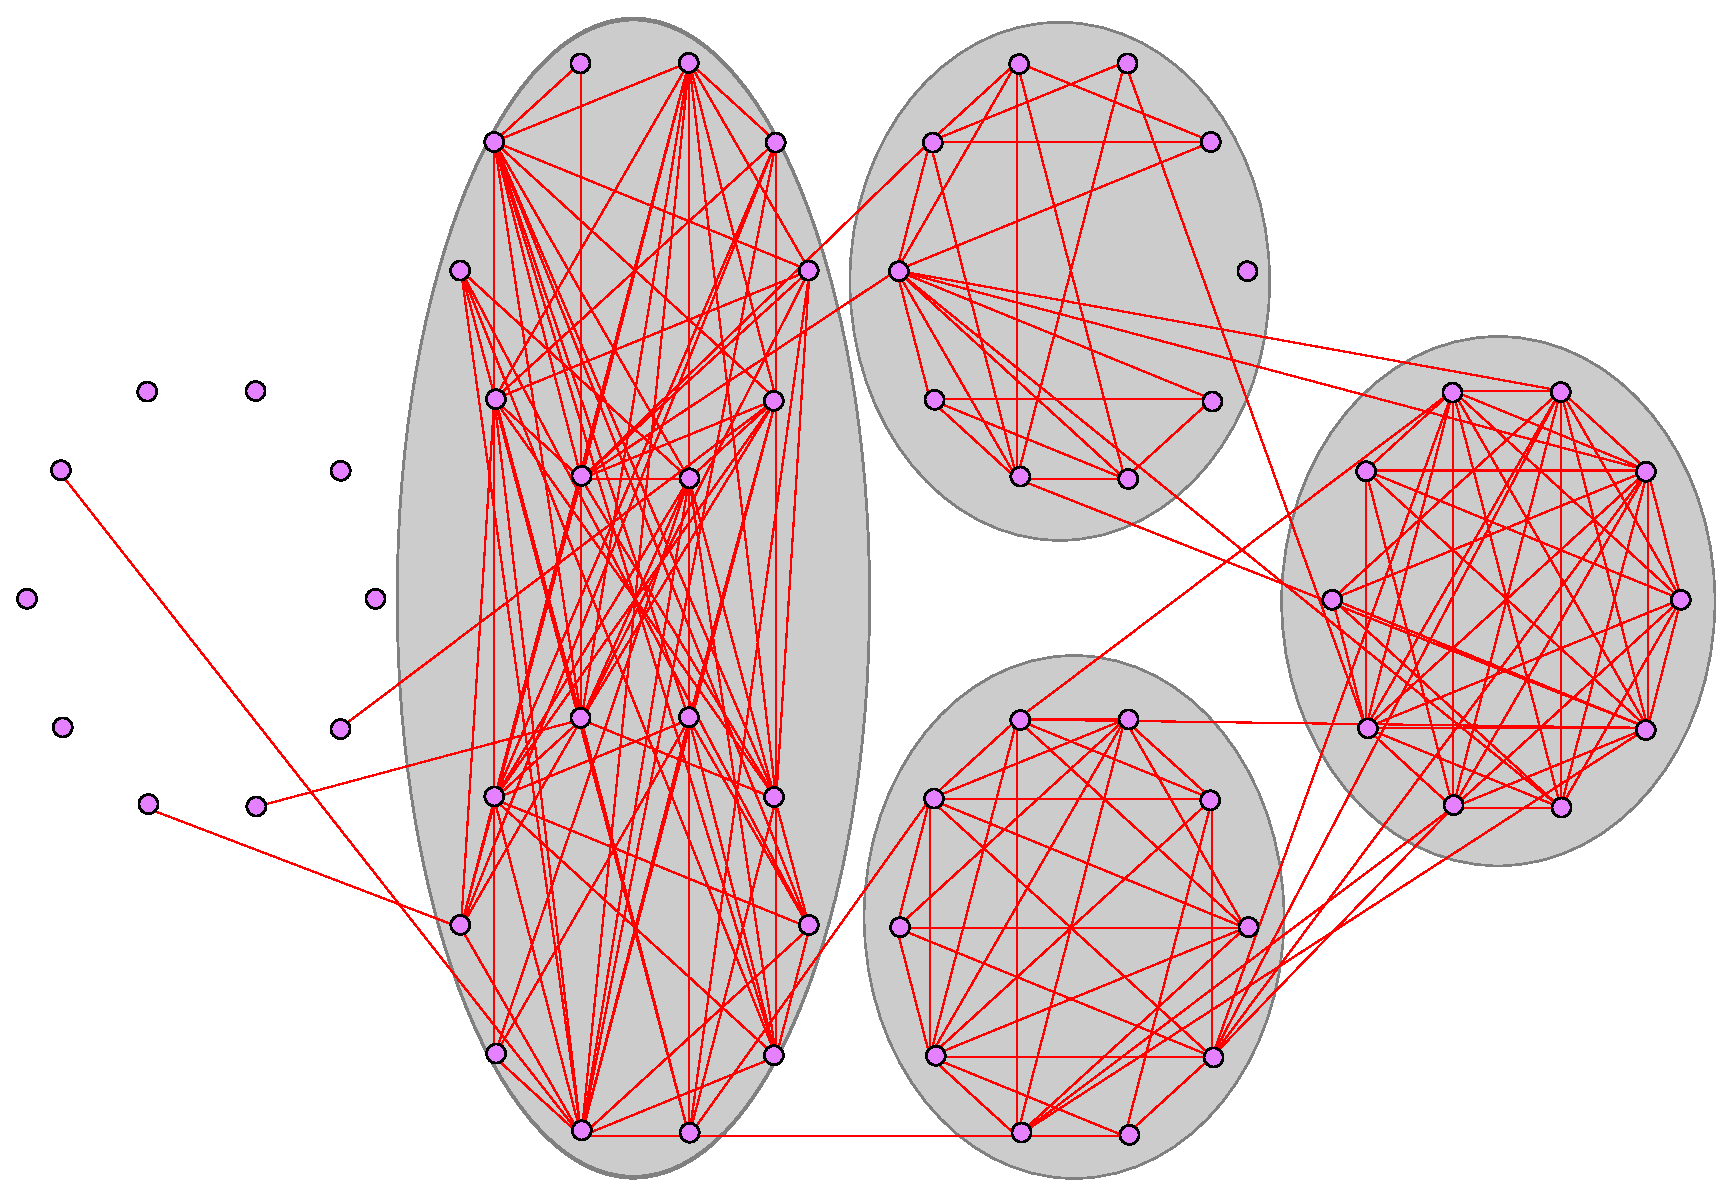
\epsfig{file=clustcocitnetnodes.eps,width=0.75\textwidth}
\end{center}
}
\section{Further Work}
\subsection{Spike-Timing Dependent Plasticity}
\frame
{
\frametitle{Another measure?}
Incremental Mutual Information gives satisfactory results, but the absolute values of the peak IMI are very low, and the computational cost is high.\pause We look for a new network measure that is easier to calculate and gives larger weights in the network.
\bigskip

\pause
Song, Miller \& Abbott [2000] suggested that neurons could learn to fire together, if the plasticity of the synapses depended on the timing of pre- and post-synaptic spikes.
\bigskip

\pause
We postulate that if there is a network structure causing the spikes, then our network could "learn" this structure through mimicking these plasticity rules.
}
\frame
{
\frametitle{Spike-Timing Dependent Plasticity}
Song, Miller and Abbott [2000] laid down the rules for spike-timing dependent plasticity (STDP) as follows:\pause
\begin{itemize}
\item<1-> Each synapse begins with plasticity $\gamma = 1$.
\pause
\item<2-> If a pre-synaptic and post-synaptic spike pair are separated by $\Delta t$ then modify $\gamma$ by $F(\Delta t)$, where:
\end{itemize}
$$
F(\Delta t) = \left\{ \begin{array}{ll} A_+ \exp (\Delta t / \tau_+) & \text{if } \Delta t>0 \\
-A_- \exp( \Delta t / \tau_-) & \text{if } \Delta t<0 \end{array} \right.
$$
\pause
If we set the values of $\tau_+=\tau_- = 20\text{ms}$ and $A_+=0.005$, $A_-=0.00525$ then the network quickly organises itself.
}

\frame
{
\frametitle{STDP as a network measure}
We alter STDP by initially setting $\gamma =0$ and letting $A_+=A_- = 0.005$ so that we get a symmetric measure.
\bigskip
\pause

Using a replica of our model network above (but with poisson spiking/noise) we get the following connectivity:
\begin{center}
\begin{tabular}{lcr}
\epsfig{file=poissonspikes.eps,height=0.3\textheight} & &\epsfig{file=stdpresult.eps,height=0.4\textheight}
\end{tabular}
\end{center}
}
\subsection{Other}
\frame
{
\begin{itemize}
\item Algebra of bibliographic and cocitation couplings.
\pause
\item Implementing a "weak" clustering as in Ball, Karrer \& Newman [2011].
\end{itemize}
}

\frame
{
\begin{center}
Questions?
\end{center}
}

\end{document}
